\subsection*{PESQUISA DE CAMPO E ANÁLISE ESTATÍSTICA}

A pesquisa de campo foi desenvolvida por meio de questionário, contendo quatro perguntas que avaliam a adoção de novas tecnologias no campo da preservação do meio ambiente. Foram feitas nove entrevistas em órgãos públicos como CETESB e Fundação Florestal, bem como um escritório de Engenharia Ambiental.
A primeira pergunta buscava conhecer se aquele órgão ou empresa estava ligado e comprometido com a preservação do meio ambiente, e foi obtido resposta positiva 100\% das entrevistas.
A segunda pergunta busca avaliar se na opinião do entrevistado, o custo envolvido na realização de um levantamento de flora, é uma barreira para usa execução. 22\% dos entrevistados responderam que não é uma barreira, enquanto os outros 78\% concordam que o custo é um fator importante na realização desse serviço.
\Cref{Gráfico 1}
\begin{figure}[!h]
    \centering
    \caption{Respostas tabuladas}
    \label{Gráfico 1}
    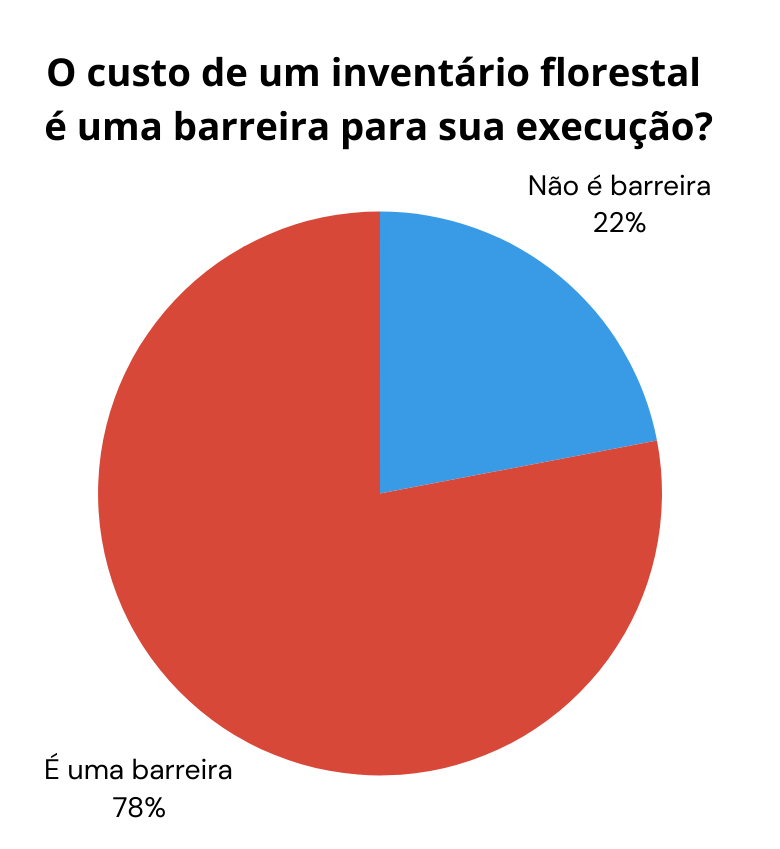
\includegraphics[width=0.5\linewidth]{Illustrations/grph-question2.png}
    \SourceOrNote{Autoria Própria (2024)}
    \end{figure}

Na terceira pergunta levantou-se a disponibilidade de ferramentas tecnológicas que auxiliem a preservação de árvores no meio ambiente. Um entrevistado respondeu que no seu setor não dispunha de quaisquer recursos, ainda que necessários. Todos os outros responderam que possuem tecnologias das mais diversas: Drones, Aerofotos, Mapa de Arborização urbana (Online), GPS, Google Earth, Sobrevoo de helicóptero, plataforma ArcGis, MITRA, Cartas Topográficas, máquina fotográfica, banco de dados diversos.
A quarta pergunta investigou o nível de confiança dos entrevistados em análises feitas por IA como auxílio para tomadas de decisão nas funções que desempenham. 44\% dos entrevistados responderam não confiar em análises feitas por IA, entretanto 56\% acreditam que ela possa ser usada como ferramenta para auxiliar tomadas de decisões.
\Cref{Gráfico 2}
\begin{figure}[!h]
    \centering
    \caption{Respostas tabuladas}
    \label{Gráfico 2}
    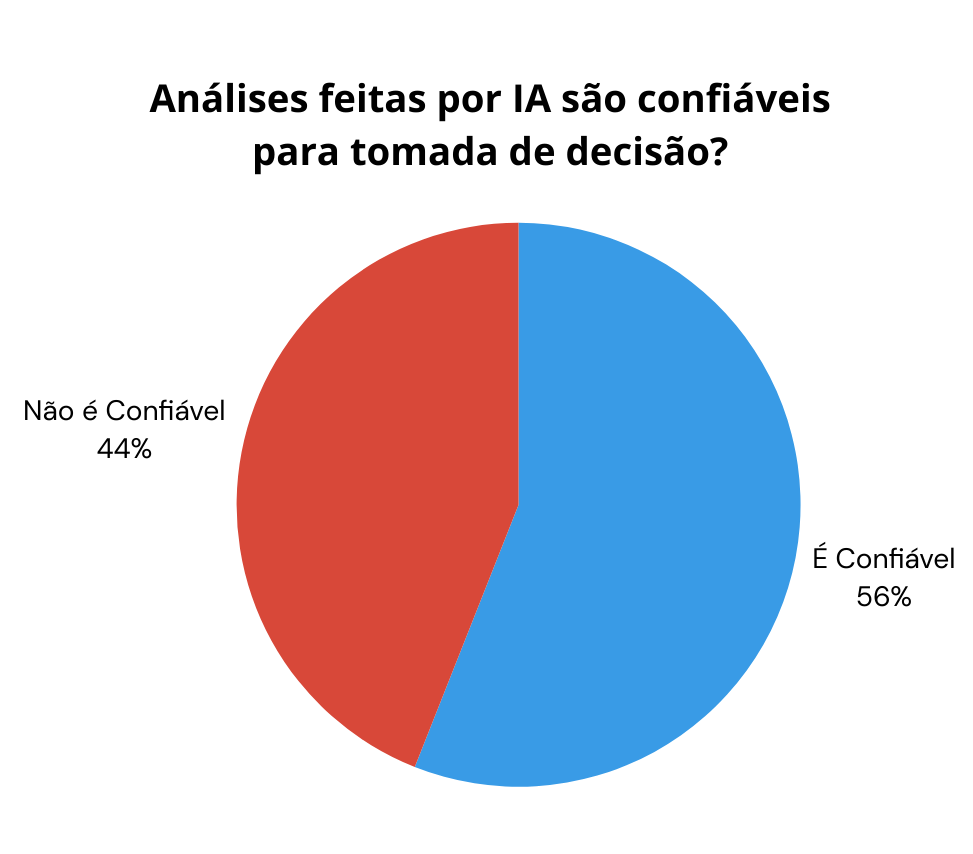
\includegraphics[width=0.65\linewidth]{Illustrations/pizza2.png}
    \SourceOrNote{Autoria Própria (2024)}
    \end{figure}

A pesquisa nos revelou que existe uma carência de ferramentas tecnológicas de monitoramento e imageamento aéreo. Isso é evidenciado no uso frequente de aerofotos antigas e cartas topográficas impressas. Pela falta desses recursos, o levantamento de espécies para um inventário florestal resulta em um serviço de alto custo, e que são feitos somente em caso de extrema necessidade. Essa situação reflete na visão que os profissionais têm sobre as IA's, em que as respostas ficaram divididas entre se elas são viáveis ou não para tomadas de decisão.

\subsection*{DESEMPENHO DO MODELO}
Resultados da Validação Cruzada
O desempenho do modelo foi avaliado utilizando validação cruzada (K-Fold Cross Validation) com 10 folds. A seguir estão os resultados de acurácia de validação para cada fold:

Fold 1: 92.5\%

Fold 2: 85.0\%

Fold 3: 85.0\%

Fold 4: 90.0\%

Fold 5: 87.5\%

Fold 6: 80.0\%

Fold 7: 82.5\%

Fold 8: 82.5\%

Fold 9: 77.5\%

Fold 10: 82.5\%

\subsubsection*{Análise da Acurácia Média}

A acurácia média de validação obtida ao longo dos 10 folds foi de 84.5\%, indicando um bom desempenho do modelo na tarefa de classificação. Esta métrica reflete a capacidade do modelo de generalizar bem para novos dados.

\subsubsection*{Variabilidade entre os Folds}

Houve alguma variação nos resultados de acurácia entre os diferentes folds, com um mínimo de 77.5\% e um máximo de 92.5\%. Esta variabilidade é esperada devido a diferenças na distribuição dos dados em cada fold e sugere que, enquanto o modelo performa consistentemente bem, há espaço para melhorias na generalização.\Cref{Gráfico 3}

O modelo foi treinado por 100 épocas com um batch size de 32, usando o otimizador Adam e a função de perda sparse\textunderscore categorical\textunderscore crossentropy. Este número de épocas foi suficiente para permitir ao modelo aprender as características dos dados sem superajustar aos dados de treinamento. A função de ativação ReLU nas camadas densas e softmax na camada de saída ajudaram a capturar relações não-lineares e a classificar corretamente as imagens.

\begin{figure}[!h]
    \centering
    \caption{Evolução da acurácia ao longo dos treinamentos}
    \label{Gráfico 3}
    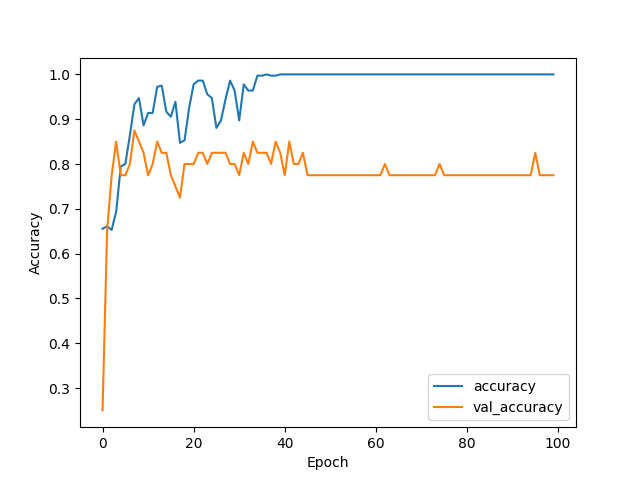
\includegraphics[width=0.7\linewidth]{Illustrations/Figure_1.png}
    \SourceOrNote{Autoria Própria (2024)}
    \end{figure}